\documentclass[10pt]{article}
\usepackage[margin=0.85in]{geometry}
\usepackage{amsmath,amssymb,graphicx,booktabs}
\usepackage[hidelinks]{hyperref}
\pagestyle{empty}
\setlength{\parskip}{4pt}\setlength{\parindent}{0pt}
\begin{document}
{\large\bfseries Gauss-Newton on $\varphi$ versus gradient descent on $f$ for globally P\L{} functions}\\[2pt]
Siddhant Gadodia, IIT Delhi \hfill \small\url{https://github.com/[USERNAME]/pl-least-squares-check}

\textbf{Setup.} Boumal, Criscitiello and Rebjock (arXiv:2604.07972) show that a smooth, globally P\L{} function on $\mathbb{R}^n$ has the form $f = f^* + \|\varphi(x)\|^2$, where $\varphi:\mathbb{R}^n\to\mathbb{R}^k$ is a submersion and $k$ is the codimension of the minimiser set $S$. I asked what this structure gives algorithmically when $\varphi$ is known: how does Gauss-Newton on $\varphi$ compare with gradient descent on $f$, and how does the gap depend on the conditioning of $D\varphi$?

\textbf{Experiment A (one dimension).} $f(x)=x^2+3\sin^2 x$ is nonconvex but P\L{}. Here $\varphi(x)=\operatorname{sign}(x)\sqrt{f(x)}$. Since $f'=2\varphi\varphi'$ and P\L{} forces $f'\neq 0$ away from $0$, $\varphi'$ cannot vanish there, and $\varphi'(0)=2$. Numerically on $[-10,10]$: $\min|\varphi'|\approx 0.296$ and $\min |f'|^2/(2f)\approx 0.176$.

\begin{center}\small
\begin{tabular}{lccccc}\toprule
start $x_0$ & $-7.3$ & $-2.1$ & $0.9$ & $3.3$ & $8.8$\\\midrule
GD on $f$ (step $1/8$) & 12 & 7 & 3 & 9 & 13\\
Gauss-Newton on $\varphi$ & 4 & 3 & 3 & 3 & 6\\\bottomrule
\end{tabular}\\[2pt] iterations to $f<10^{-10}$
\end{center}

\textbf{Experiment B (conditioning).} $\varphi(x)=Ax+0.3\sin(Bx)$ from $\mathbb{R}^{20}$ to $\mathbb{R}^5$, with $A$ of condition number $\kappa$. Both methods use Armijo backtracking. Gauss-Newton uses the minimum-norm step $-D\varphi^{+}\varphi$ since $k<n$. Median over five random starts.

\begin{minipage}{0.42\textwidth}\centering\small
\begin{tabular}{rcc}\toprule
$\kappa$ & GD & Gauss-Newton\\\midrule
1 & 12 & 3\\ 3 & 46 & 4\\ 10 & 136 & 3\\ 30 & 214 & 4\\ 100 & 303 & 4\\\bottomrule
\end{tabular}
\end{minipage}\hfill
\begin{minipage}{0.55\textwidth}\centering
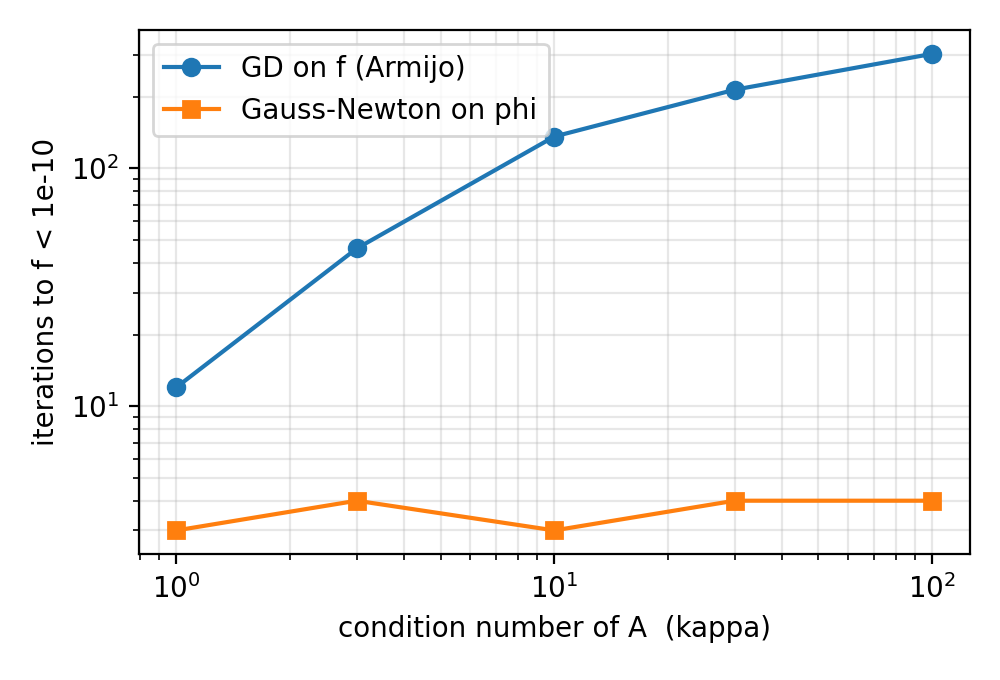
\includegraphics[width=0.92\linewidth]{pl_gd_vs_gn.png}
\end{minipage}

\textbf{Observations.}
(1) On $S$, $\nabla^2 f = 2\,D\varphi^\top D\varphi$, so near $S$ Gauss-Newton on $\varphi$ coincides with Newton on $f$. The comparison is only informative away from $S$.
(2) Iteration counts understate the cost of Gauss-Newton, which needs a least-squares solve per step.
(3) These results are expected once $\varphi$ is known. The open part, for me, is that $\varphi$ is usually not available. In the paper it arises from the gradient flow, which raises the question of whether a computable approximation of $\varphi$ away from $S$ could serve as a preconditioner for first-order methods.

\end{document}
